\documentclass[aspectratio=169]{beamer}

\usepackage{../theme}
\usepackage{../boxes}

\title{\textbf{\Huge Krypto Währungen}}
\author{\textcolor{secondarycolor}{\textbf{Christian Laussmann}}}
\date{}

\begin{document}

\frame{\titlepage}





\section{Einführung}


\begin{frame}{Bargeldzahlung}
    \begin{center}
        \begin{tabular}{ccccc}
            
\includegraphics[width=2.5cm]{../icons/Alan} & {\Huge$\longrightarrow$} & 
\includegraphics[width=2cm]{../icons/Coin} & {\Huge$\longrightarrow$} & 
\includegraphics[width=2.5cm]{../icons/Linus}\\
            Alan & & & & Linus\\
        \end{tabular}
    \end{center}
    \vspace{0.5cm}

    \pause
    \textbf{Das funktioniert, weil:}
    \begin{itemize}
        \item Alan \textbf{besitzt} die Münze und \textbf{darf} sie abgeben.
        \item Linus \textbf{besitzt} anschließend die Münze und kann damit bezahlen.
        \item Alan kann Linus die Münze nicht \textbf{wegnehmen} oder die Münze \textbf{erneut ausgeben}.
    \end{itemize}
\end{frame}



\begin{frame}{Überweisung}
    \begin{center}
        \begin{tabular}{ccccc}
            
\includegraphics[width=2cm]{../icons/Alan}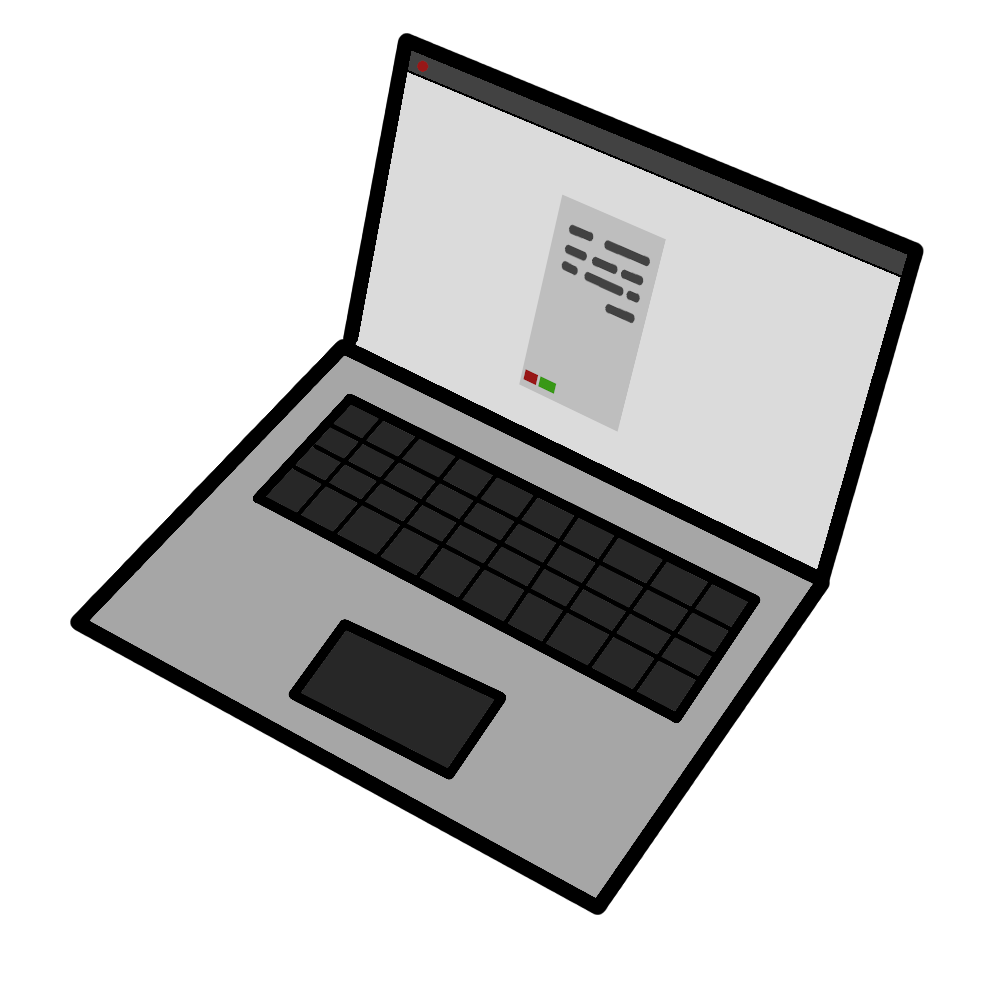
\includegraphics[width=1.5cm]{../icons/ComputerLeft} & {\Huge$\longrightarrow$} & 
\includegraphics[width=2.5cm]{../icons/Bank} & {\Huge$\longrightarrow$} & 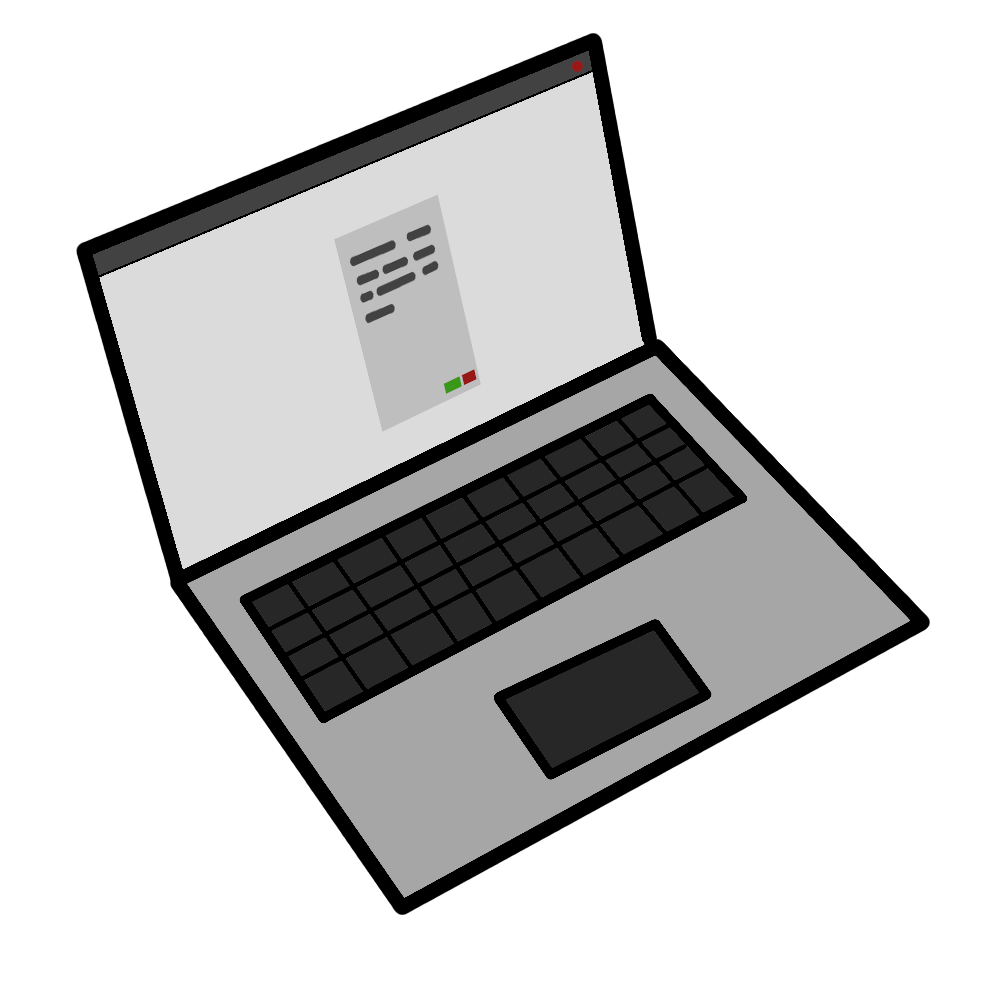
\includegraphics[width=1.5cm]{../icons/ComputerRight}
\includegraphics[width=2cm]{../icons/Linus}\\
            Alan & & Prüfung durch Bank & & Linus\\
        \end{tabular}
    \end{center}
    \vspace{0.5cm}

    \pause
    \begin{itemize}
        \item \textbf{Gültigkeit:} Alans Bank prüft Alans Kontostand. Gesetze und Zentralbanken verhindern Betrug zwischen den Banken.
        \item \textbf{Authorisierung:} Alan hat Zugangsdaten zum Onlinebanking.
        \item \textbf{Unveränderlichkeit:} Sichergestellt durch Gesetze und Zentralbanken.
    \end{itemize}
\end{frame}



\begin{frame}{Krypto-Überweisung}
    \begin{center}
        \begin{tabular}{ccccc}
            
\includegraphics[width=2cm]{../icons/Alan}\hspace*{-0.5cm}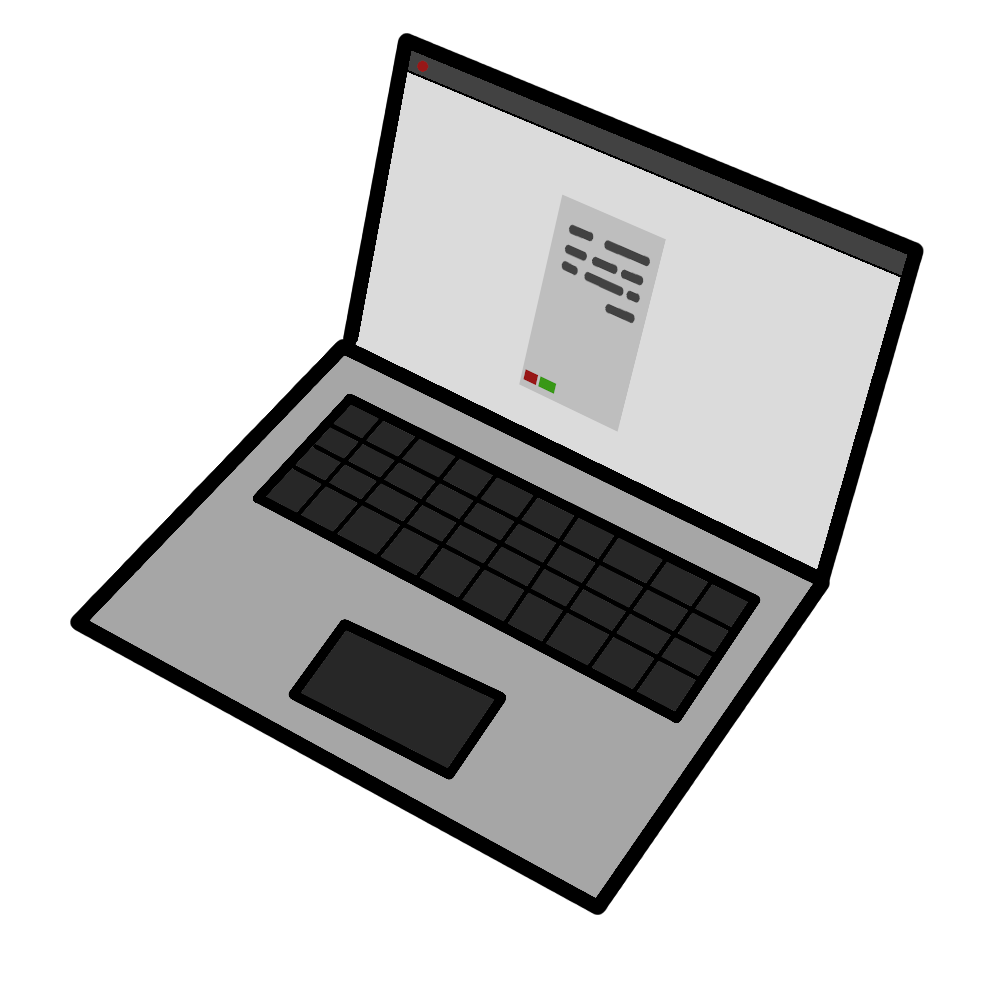
\includegraphics[width=1.5cm]{../icons/ComputerLeft} & {\Huge$\longrightarrow$} & 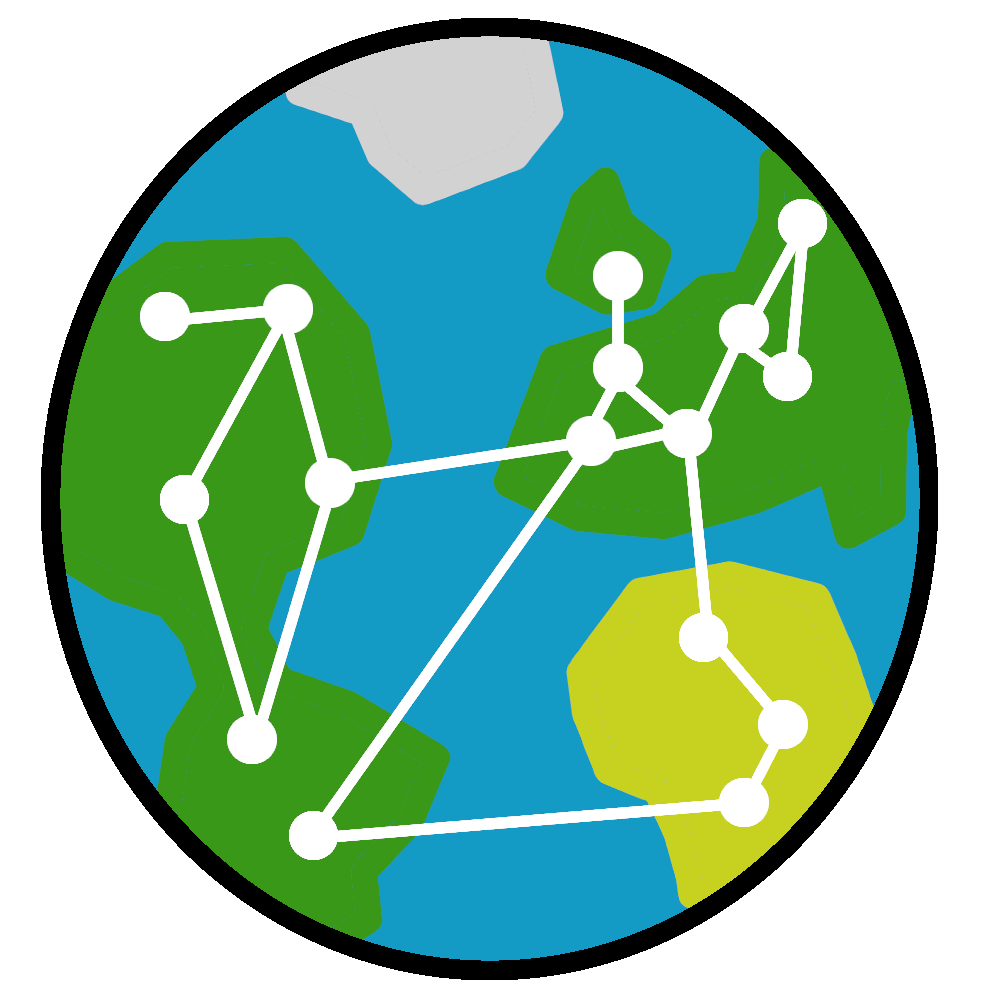
\includegraphics[width=2.5cm]{../icons/Internet}\hspace*{-1.5cm}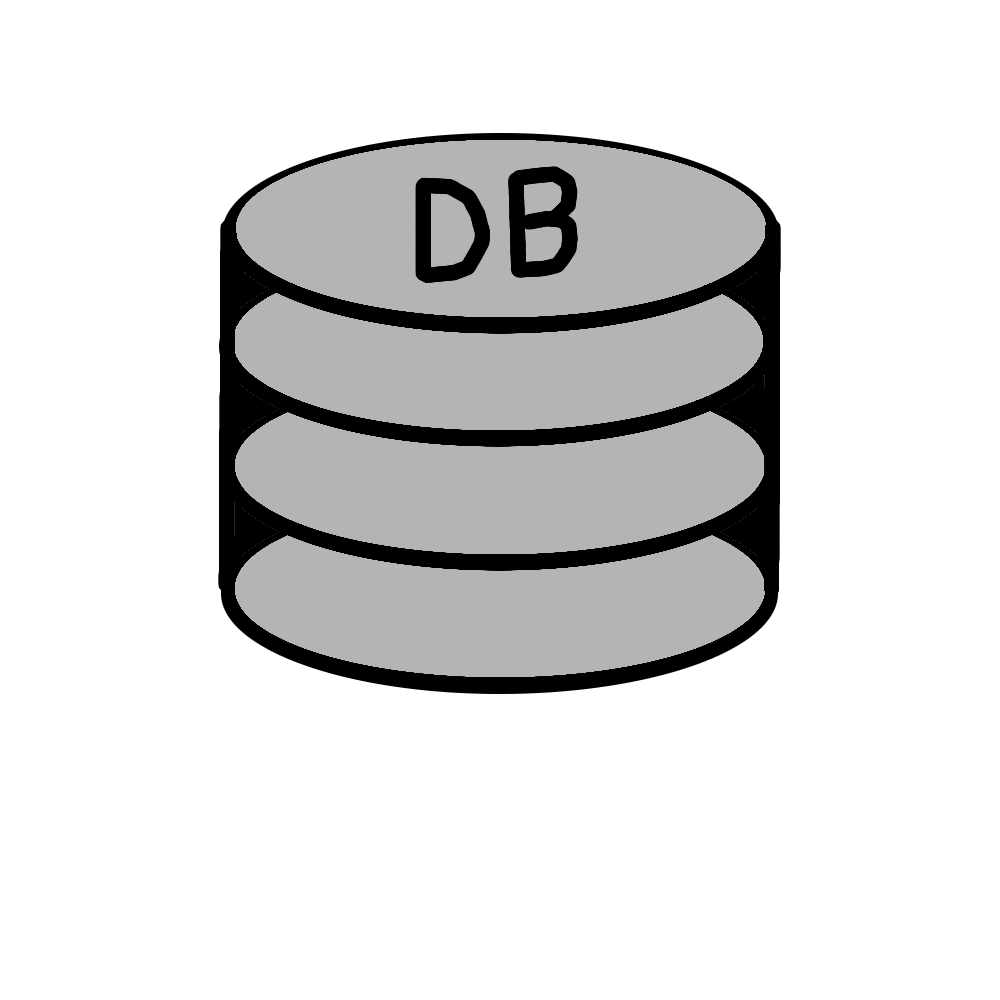
\includegraphics[width=2cm]{../icons/DB} & {\Huge$\longrightarrow$} & 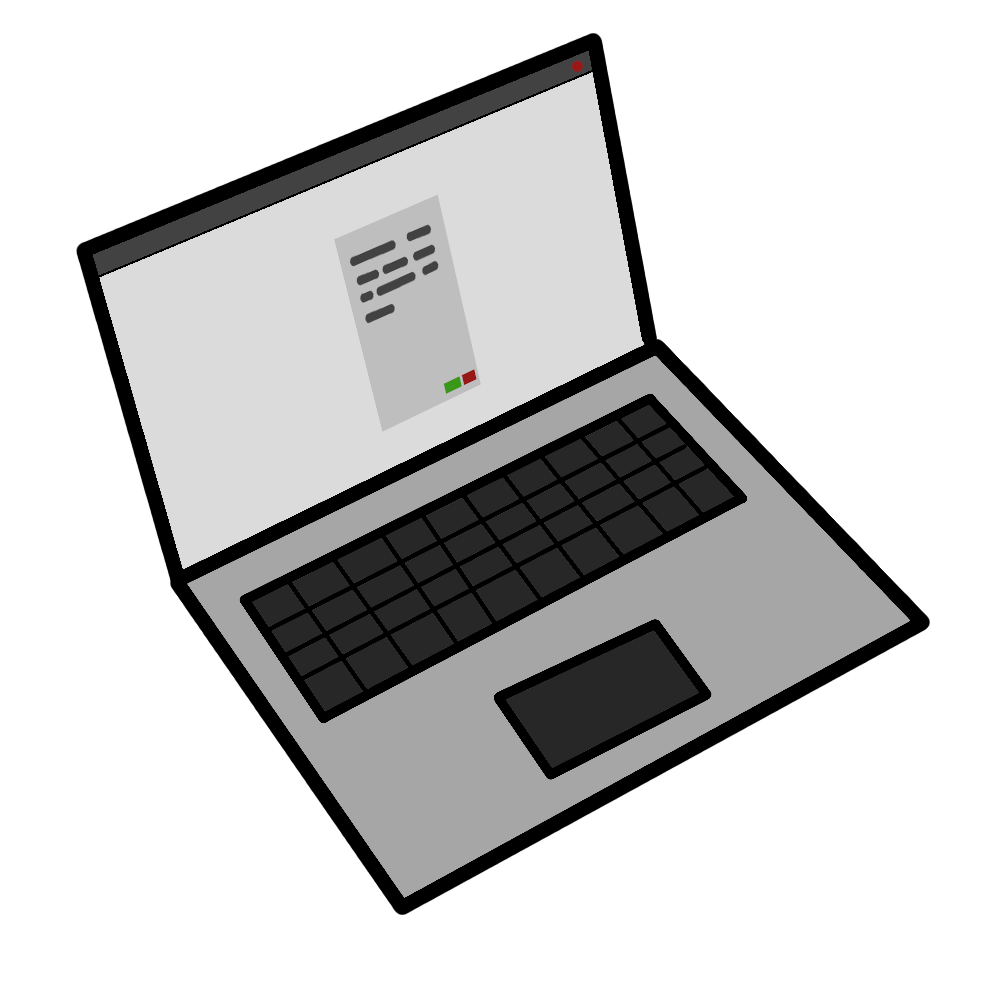
\includegraphics[width=1.5cm]{../icons/ComputerRight}\hspace*{-0.5cm}
\includegraphics[width=2cm]{../icons/Linus}\\
            Alan & & ``Alan sendet Linus 
\includegraphics[width=0.5cm]{../icons/Coin}'' & & Linus\\
        \end{tabular}
    \end{center}
    \vspace{0.5cm}

    \pause
    \begin{itemize}
        \item \textbf{Gültigkeit:} Wer prüft, ob Alan genug Geld hat?
        \item \textbf{Authorisierung:} Wie ist garantiert, dass jeder nur eigenes Geld überweisen kann?
        \item \textbf{Unveränderlichkeit:} Wer garantiert, dass Transaktionen nicht bearbeitet werden?
        \item \textbf{Niemand vertraut den anderen -- nur der Mathematik.}
    \end{itemize}
\end{frame}


\section{Unveränderlichkeit}
\includesectiontitle

\begin{frame}[fragile]{Die Blockchain}
    \begin{center}
        \boxwithtitle{3.85cm}{a}{Block \#1}{
            Transaktion 1\\
            Transaktion 2\\
            ...
        }
        \hspace{0.7cm}
        \boxwithtitle{3.85cm}{b}{Block \#2}{
            Transaktion 3\\
            Transaktion 4\\
            ...
        }
        \hspace{0.7cm}
        \boxwithtitle{3.85cm}{c}{Block \#3}{
            Transaktion 7\\
            Transaktion 8\\
            ...
        }
    \end{center}
    \begin{tikzpicture}[overlay, remember picture]
        \draw[->, line width=2pt] (b) -- (a);
        \draw[->, line width=2pt] (c) -- (b);
    \end{tikzpicture}
\end{frame}


\begin{frame}{Hash-Pointer}
    \begin{center}
        \boxwithtitle{3.85cm}{a}{c6cc}{
            Vorgänger: null\\
            Transaktionen:\\
            ...
        }
        \hspace{0.7cm}
        \boxwithtitle{3.85cm}{b}{afaa}{
            Vorgänger: \textbf{c6cc}\\
            Transaktionen:\\
            ...
        }
        \hspace{0.7cm}
        \boxwithtitle{3.85cm}{c}{7ffa}{
            Vorgänger: \textbf{afaa}\\
            Transaktionen:\\
            ...
        }
    \end{center}
    \begin{tikzpicture}[overlay, remember picture]
        \draw[->, line width=2pt] (b) -- (a);
        \draw[->, line width=2pt] (c) -- (b);
    \end{tikzpicture}
    \pause

    \terminalbox{christian@dev \$\_}{
        \$\_\;\; echo 'Hallo Christian' | sha256sum\\
        \phantom{...} 37c24999d0c3f6b0d295c19699bc121c6b7c194fb957b15bdb3582c60edf3a1f\\~\\
        \$\_\;\; echo 'hallo christian' | sha256sum\\
        \phantom{...} e52c859ed0b18b5dcce6d177caf000b19c7c578504f9dbc626580387b1f79ab5
    }
\end{frame}


\begin{frame}{Gebrochene Kette}
    \begin{center}
        \boxwithtitle{3.85cm}{a}{c6cc}{
            Vorgänger: null\\
            Transaktionen:\\
            ...
        }
        \hspace{0.7cm}
        \boxwithtitle{3.85cm}{b}{\textcolor{myviolet}{afaa}}{
            Vorgänger: \textbf{c6cc}\\
            Transaktionen:\\
            \textcolor{myviolet}{\textbf{Alan sendet 4}}
        }
        \hspace{0.7cm}
        \boxwithtitle{3.85cm}{c}{7ffa}{
            Vorgänger: \textbf{\textcolor{myviolet}{afaa}}\\
            Transaktionen:\\
            ...
        }
    \end{center}
    \begin{tikzpicture}[overlay, remember picture]
        \draw[->, line width=2pt] (b) -- (a);
        \draw[->, line width=2pt] (c) -- (b);
    \end{tikzpicture}

    \pause
    \begin{center}
        \boxwithtitle{3.85cm}{e}{c6cc}{
            Vorgänger: null\\
            Transaktionen:\\
            ...
        }
        \hspace{0.7cm}
        \boxwithtitle{3.85cm}{f}{\textcolor{myblue}{6ae7}}{
            Vorgänger: \textbf{c6cc}\\
            Transaktionen:\\
            \textcolor{myblue}{\textbf{Alan sendet 1}}
        }
        \hspace{0.7cm}
        \boxwithtitle{3.85cm}{g}{7ffa}{
            Vorgänger: \textbf{\textcolor{myviolet}{afaa}}\\
            Transaktionen:\\
            ...
        }
    \end{center}
    \begin{tikzpicture}[overlay, remember picture]
        \draw[->, line width=2pt] (f) -- (e);
        \draw[->, dashed, line width=2pt, color=myred] (g) -- (f);
    \end{tikzpicture}
\end{frame}


\begin{frame}{Reparatur einer gebrochenen Kette}
    \begin{center}
        \boxwithtitle{3.85cm}{a}{c6cc}{
            Vorgänger: null\\
            Transaktionen:\\
            ...
        }
        \hspace{0.7cm}
        \boxwithtitle{3.85cm}{b}{\textcolor{myblue}{6ae7}}{
            Vorgänger: \textbf{c6cc}\\
            Transaktionen:\\
            \textcolor{myblue}{\textbf{Alan sendet 1}}
        }
        \hspace{0.7cm}
        \boxwithtitle{3.85cm}{c}{7ffa}{
            Vorgänger: \textbf{\textcolor{myviolet}{afaa}}\\
            Transaktionen:\\
            ...
        }

        \vspace{1.5cm}

        \boxwithtitle{3.85cm}{e}{22ea}{
            Vorgänger: \textbf{5aff}\\
            Transaktionen:\\
            ...
        }
        \hspace{0.7cm}
        \boxwithtitle{3.85cm}{d}{5aff}{
            Vorgänger: \textbf{7ffa}\\
            Transaktionen:\\
            ...
        }
    \end{center}
    \begin{tikzpicture}[overlay, remember picture]
        \draw[->, line width=2pt] (b) -- (a);
        \draw[->, dashed, line width=2pt, color=myred] (c) -- (b);
        \draw[->, line width=2pt] (d) -- (c);
        \draw[->, line width=2pt] (e) -- (d);
    \end{tikzpicture}
\end{frame}

\begin{frame}{Reparatur einer gebrochenen Kette}
    \begin{center}
        \boxwithtitle{3.85cm}{a}{c6cc}{
            Vorgänger: null\\
            Transaktionen:\\
            ...
        }
        \hspace{0.7cm}
        \boxwithtitle{3.85cm}{b}{\textcolor{myblue}{6ae7}}{
            Vorgänger: \textbf{c6cc}\\
            Transaktionen:\\
            \textcolor{myblue}{\textbf{Alan sendet 1}}
        }
        \hspace{0.7cm}
        \boxwithtitle{3.85cm}{c}{\textcolor{myblue}{dad4}}{
            Vorgänger: \textbf{\textcolor{myblue}{6ae7}}\\
            Transaktionen:\\
            ...
        }

        \vspace{1.5cm}

        \boxwithtitle{3.85cm}{e}{22ea}{
            Vorgänger: \textbf{5aff}\\
            Transaktionen:\\
            ...
        }
        \hspace{0.7cm}
        \boxwithtitle{3.85cm}{d}{5aff}{
            Vorgänger: \textbf{\textcolor{myviolet}{7ffa}}\\
            Transaktionen:\\
            ...
        }
    \end{center}
    \begin{tikzpicture}[overlay, remember picture]
        \draw[->, line width=2pt] (b) -- (a);
        \draw[->, line width=2pt] (c) -- (b);
        \draw[->, dashed, line width=2pt, color=myred] (d) -- (c);
        \draw[->, line width=2pt] (e) -- (d);
    \end{tikzpicture}
\end{frame}

\begin{frame}{Reparatur einer gebrochenen Kette}
    \begin{center}
        \boxwithtitle{3.85cm}{a}{c6cc}{
            Vorgänger: null\\
            Transaktionen:\\
            ...
        }
        \hspace{0.7cm}
        \boxwithtitle{3.85cm}{b}{\textcolor{myblue}{6ae7}}{
            Vorgänger: \textbf{c6cc}\\
            Transaktionen:\\
            \textcolor{myblue}{\textbf{Alan sendet 1}}
        }
        \hspace{0.7cm}
        \boxwithtitle{3.85cm}{c}{\textcolor{myblue}{dad4}}{
            Vorgänger: \textbf{\textcolor{myblue}{6ae7}}\\
            Transaktionen:\\
            ...
        }

        \vspace{1.5cm}

        \boxwithtitle{3.85cm}{e}{22ea}{
            Vorgänger: \textbf{\textcolor{myviolet}{5aff}}\\
            Transaktionen:\\
            ...
        }
        \hspace{0.7cm}
        \boxwithtitle{3.85cm}{d}{\textcolor{myblue}{85a7}}{
            Vorgänger: \textbf{\textcolor{myblue}{dad4}}\\
            Transaktionen:\\
            ...
        }
    \end{center}
    \begin{tikzpicture}[overlay, remember picture]
        \draw[->, line width=2pt] (b) -- (a);
        \draw[->, line width=2pt] (c) -- (b);
        \draw[->, line width=2pt] (d) -- (c);
        \draw[->, dashed, line width=2pt, color=myred] (e) -- (d);
    \end{tikzpicture}
\end{frame}

\begin{frame}{Nonce und Hash-Challenge}
    \begin{center}
        \boxwithtitle{3.85cm}{a}{00a4}{
            Nonce: 42\\
            Vorgänger: null\\
            Transaktionen:\\
            ...
        }
        \hspace{0.7cm}
        \boxwithtitle{3.85cm}{b}{002e}{
            Nonce: 7736\\
            Vorgänger: \textbf{00a4}\\
            Transaktionen:\\
            ...
        }
        \hspace{0.7cm}
        \boxwithtitle{3.85cm}{c}{00fa}{
            Nonce: 4322\\
            Vorgänger: \textbf{002e}\\
            Transaktionen:\\
            ...
        }
    \end{center}
    \begin{tikzpicture}[overlay, remember picture]
        \draw[->, line width=2pt] (b) -- (a);
        \draw[->, line width=2pt] (c) -- (b);
    \end{tikzpicture}
    \begin{itemize}
        \item Wir akzeptieren nur Hash-Werte mit mindestens $X$ Nullen
        \item Passende Nonce durch ausprobieren finden \textbf{(\emph{Mining})}
    \end{itemize}
\end{frame}

\begin{frame}{Hash-Challenge}
    \terminalbox{christian@dev \$\_}{
        \$\_\;\; echo '\textbf{Alan sendet 3. \textcolor{myblue}{Nonce: 737}. Vorgänger: 00af}' | sha256sum\\
        \phantom{...} \textcolor{myviolet}{96c7...}\\~\\\pause
        \$\_\;\; echo '\textbf{Alan sendet 3. \textcolor{myblue}{Nonce: 325}. Vorgänger: 00af}' | sha256sum\\
        \phantom{...} \textcolor{myviolet}{b95a...}\\~\\\pause
        \$\_\;\; echo '\textbf{Alan sendet 3. \textcolor{myblue}{Nonce: 129}. Vorgänger: 00af}' | sha256sum\\
        \phantom{...} \textcolor{myviolet}{0ad2...}\\~\\\pause
        \$\_\;\; echo '\textbf{Alan sendet 3. \textcolor{myblue}{Nonce: 729}. Vorgänger: 00af}' | sha256sum\\
        \phantom{...} \textcolor{myviolet}{101d...}\\
        ...
    }
\end{frame}

\begin{frame}{Fazit bis hier}
    \begin{center}
        \boxwithtitle{3.85cm}{a}{00a4}{
            Nonce: 43732\\
            Vorgänger: null\\
            Transaktionen:\\
            ...
        }
        \hspace{0.7cm}
        \boxwithtitle{3.85cm}{b}{\textcolor{myred}{af3f}}{
            Nonce: 77236\\
            Vorgänger: \textbf{00a4}\\
            Transaktionen:\\
            \textcolor{myred}{\textbf{Alan sendet 1}}
        }
        \hspace{0.7cm}
        \boxwithtitle{3.85cm}{c}{000a}{
            Nonce: 9776762\\
            Vorgänger: \textbf{\textcolor{myred}{006b}}\\
            Transaktionen:\\
            ...
        }

        \vspace{1cm}

        \boxwithtitle{3.85cm}{e}{009d}{
            Nonce: 42\\
            Vorgänger: \textbf{00e3}\\
            Transaktionen:\\
            ...
        }
        \hspace{0.7cm}
        \boxwithtitle{3.85cm}{d}{00e3}{
            Nonce: 334221\\
            Vorgänger: \textbf{000a}\\
            Transaktionen:\\
            ...
        }
    \end{center}
    \begin{tikzpicture}[overlay, remember picture]
        \draw[->, line width=2pt] (b) -- (a);
        \draw[->, dashed, line width=2pt, color=myred] (c) -- (b);
        \draw[->, line width=2pt] (d) -- (c);
        \draw[->, line width=2pt] (e) -- (d);
    \end{tikzpicture}
\end{frame}





\section{Authorisierung}
\includesectiontitle

\begin{frame}{Accounterstellung}
    \begin{center}
        \begin{tabular}{ccccc}
            
\includegraphics[width=2cm]{../icons/Linus} & {\Huge$\longrightarrow$} & 
\includegraphics[width=1.5cm]{../icons/PubKey} \hspace*{-0.5cm} 
\includegraphics[width=1.5cm]{../icons/SecKey} & {\Huge$\longrightarrow$} & {\Huge Hash(
\includegraphics[width=1.5cm]{../icons/PubKey})}\\~\\
            Linus & erzeugt & & veröffentlicht & Kontonummer\\
        \end{tabular}
    \end{center}
\end{frame}


\begin{frame}{Überweisung Authorisieren}
    \begin{center}
        \begin{tabular}{ccl}
            
\includegraphics[width=2cm]{../icons/Linus} \hspace*{-0.5cm} 
\includegraphics[width=1cm]{../icons/SecKey} & {\Huge$\longrightarrow$} & \textbf{TX =} ``Überweise 
\includegraphics[width=0.5cm]{../icons/Coin} an bc1qy3...'',\\
            & & \textbf{Sig(
\includegraphics[width=0.5cm]{../icons/SecKey}, TX)}, 
\includegraphics[width=0.5cm]{../icons/PubKey}\\
        \end{tabular}
    \end{center}
    \vspace{1cm}
    \begin{itemize}
        \item Jeder kann mittels 
\includegraphics[width=0.5cm]{../icons/PubKey} prüfen, dass \textbf{Sig(
\includegraphics[width=0.5cm]{../icons/SecKey}, TX)} gültig ist.
        \item Kontonummer ist eindeutig mit 
\includegraphics[width=0.5cm]{../icons/PubKey} verknüpft.
    \end{itemize}
\end{frame}





\section{Gültigkeit}
\includesectiontitle

\begin{frame}{Wann ist Transaktion gültig?}
    \textbf{TX = ``Überweise 
\includegraphics[width=0.5cm]{../icons/Coin} an bc1qy3...''}\\~\\
    \begin{itemize}
        \item Transaktion authorisiert? $\Rightarrow$ Signatur \textcolor{mydarkgreen}{\Large\checkmark}
        \item Kontostand ausreichend?
    \end{itemize}
\end{frame}


\begin{frame}{Prüfen des Kontostands}
    \begin{center}
        \boxwithtitle{3.85cm}{a}{c6cc}{
            b6e $\rightarrow$ 
\includegraphics[width=0.5cm]{../icons/Coin} \textcolor{myviolet}{\textbf{a5e}}\\
            ee4 $\rightarrow$ 
\includegraphics[width=0.5cm]{../icons/Coin} 3d2\\
            ...
        }
        \hspace{0.7cm}
        \boxwithtitle{3.85cm}{b}{afaa}{
            \textcolor{myviolet}{\textbf{a5e}} $\rightarrow$ 
\includegraphics[width=0.5cm]{../icons/Coin} cc7\\
            4ed $\rightarrow$ 
\includegraphics[width=0.5cm]{../icons/Coin} 95a\\
            ...
        }
        \hspace{0.7cm}
        \boxwithtitle{3.85cm}{c}{7ffa}{
            95a $\rightarrow$ 
\includegraphics[width=0.5cm]{../icons/Coin} aed\\
            e5e $\rightarrow$ 
\includegraphics[width=0.5cm]{../icons/Coin} cf2\\
            ...
        }
    \end{center}
    \begin{tikzpicture}[overlay, remember picture]
        \draw[->, line width=2pt] (b) -- (a);
        \draw[->, line width=2pt] (c) -- (b);
    \end{tikzpicture}
    \vspace{0.75cm}
    \textbf{TX = ``\textcolor{myviolet}{\textbf{a5e}} $\rightarrow$ 
\includegraphics[width=0.5cm]{../icons/Coin} cc7''}
    \begin{itemize}
        \item Transaktion authorisiert? $\Rightarrow$ Signatur \textcolor{mydarkgreen}{\Large\checkmark}
        \item Kontostand ausreichend? $\Rightarrow$ Suchen ob Geld auf Konto \textcolor{mydarkgreen}{\Large\checkmark}
    \end{itemize}
\end{frame}


\begin{frame}{Verhindern von \emph{Double-Spent}}
    \begin{center}
        \boxwithtitle{3.85cm}{a}{c6cc}{
            b6e $\rightarrow$ 
\includegraphics[width=0.5cm]{../icons/Coin} \textcolor{myviolet}{\textbf{a5e}}\\
            ee4 $\rightarrow$ 
\includegraphics[width=0.5cm]{../icons/Coin} 3d2\\
            ...
        }
        \hspace{0.7cm}
        \boxwithtitle{3.85cm}{b}{afaa}{
            \textcolor{myviolet}{\textbf{a5e}} $\rightarrow$ 
\includegraphics[width=0.5cm]{../icons/Coin} cc7\\
            4ed $\rightarrow$ 
\includegraphics[width=0.5cm]{../icons/Coin} 95a\\
            ...
        }
        \hspace{0.7cm}
        \boxwithtitle{3.85cm}{c}{7ffa}{
            \textcolor{myviolet}{\textbf{a5e}} $\rightarrow$ 
\includegraphics[width=0.5cm]{../icons/Coin} bb6\\
            e5e $\rightarrow$ 
\includegraphics[width=0.5cm]{../icons/Coin} cf2\\
            ...
        }
    \end{center}
    \begin{tikzpicture}[overlay, remember picture]
        \draw[->, line width=2pt] (b) -- (a);
        \draw[->, line width=2pt] (c) -- (b);
    \end{tikzpicture}
    \vspace{0.75cm}
    \textbf{TX = ``\textcolor{myviolet}{\textbf{a5e}} $\rightarrow$ 
\includegraphics[width=0.5cm]{../icons/Coin} cc7''}
    \begin{itemize}
        \item Transaktion authorisiert? $\Rightarrow$ Signatur \textcolor{mydarkgreen}{\Large\checkmark}
        \item Kontostand ausreichend? $\Rightarrow$ Geld bereits ausgegeben \textcolor{myred}{\Large X}
    \end{itemize}
\end{frame}


\begin{frame}{Fazit bis hier}
    \begin{itemize}
        \item \textbf{Blockchain und Nonce:} Transaktionen sind unveränderlich
        \item \textbf{Signaturen:} Nur Eigentümer kann Überweisen
        \item \textbf{Block-Historie:} Kontostand prüfen
    \end{itemize}
    \vspace{1cm}
    \pause
    \textbf{Offene Fragen:}
    \begin{itemize}
        \item Wer prüft das?
        \item Wer erstellt neue Blöcke?
        \item Woher kommen die Coins ursprünglich?
    \end{itemize}
\end{frame}


\section{Mining}
\includesectiontitle

\begin{frame}{Blöcke erschaffen}
    \begin{center}
        \begin{tabular}{ccccc}
            TX1, TX2, TX3, ... & {\Huge$\longrightarrow$} & 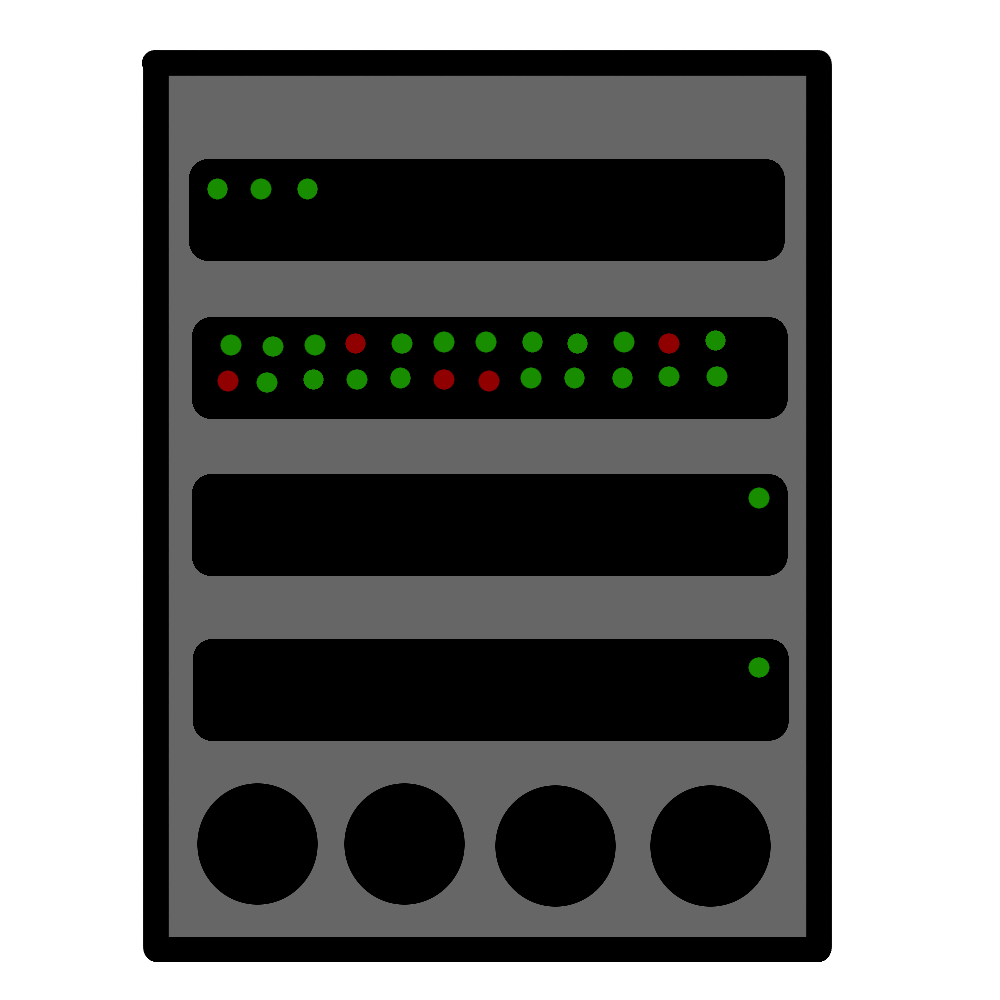
\includegraphics[width=2.5cm]{../icons/Server} & {\Huge$\longrightarrow$} & \boxwithtitle{3.25cm}{c}{7ffa}{Vorgänger, Nonce, TX1, TX2, TX3, ...}\\
            & & Sammeln, Prüfen, &\\
            & & Nonce finden, &\\
            & & \emph{\textbf{(Mining)}} &\\
        \end{tabular}
    \end{center}
\end{frame}


\begin{frame}{Woher kommt das Geld?}
    \begin{center}
        \begin{tabular}{ccccc}
            TX1, TX2, TX3, ... & {\Huge$\longrightarrow$} & 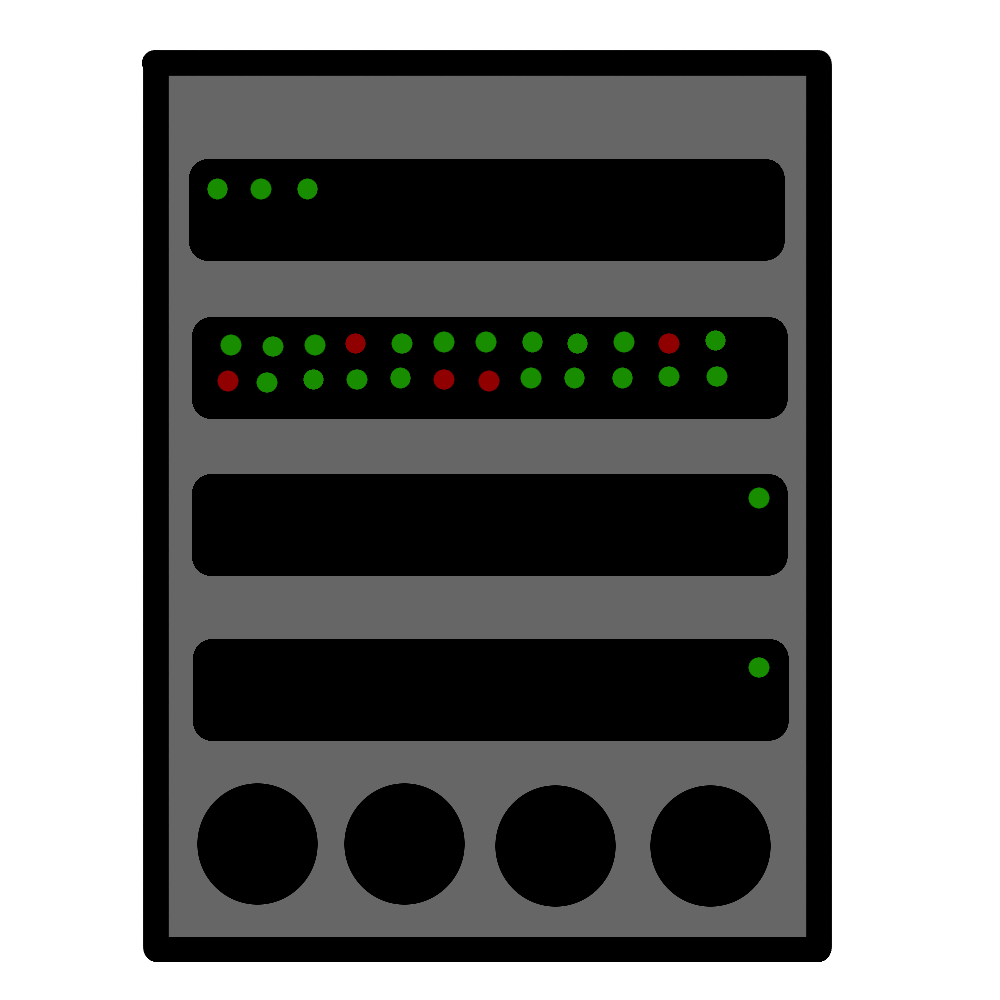
\includegraphics[width=2.5cm]{../icons/Server} & {\Huge$\longrightarrow$} & \boxwithtitle{3.25cm}{c}{7ffa}{Vorgänger, Nonce, TX1, TX2, TX3, ..., 
\includegraphics[width=0.5cm]{../icons/Coin} $\rightarrow$ 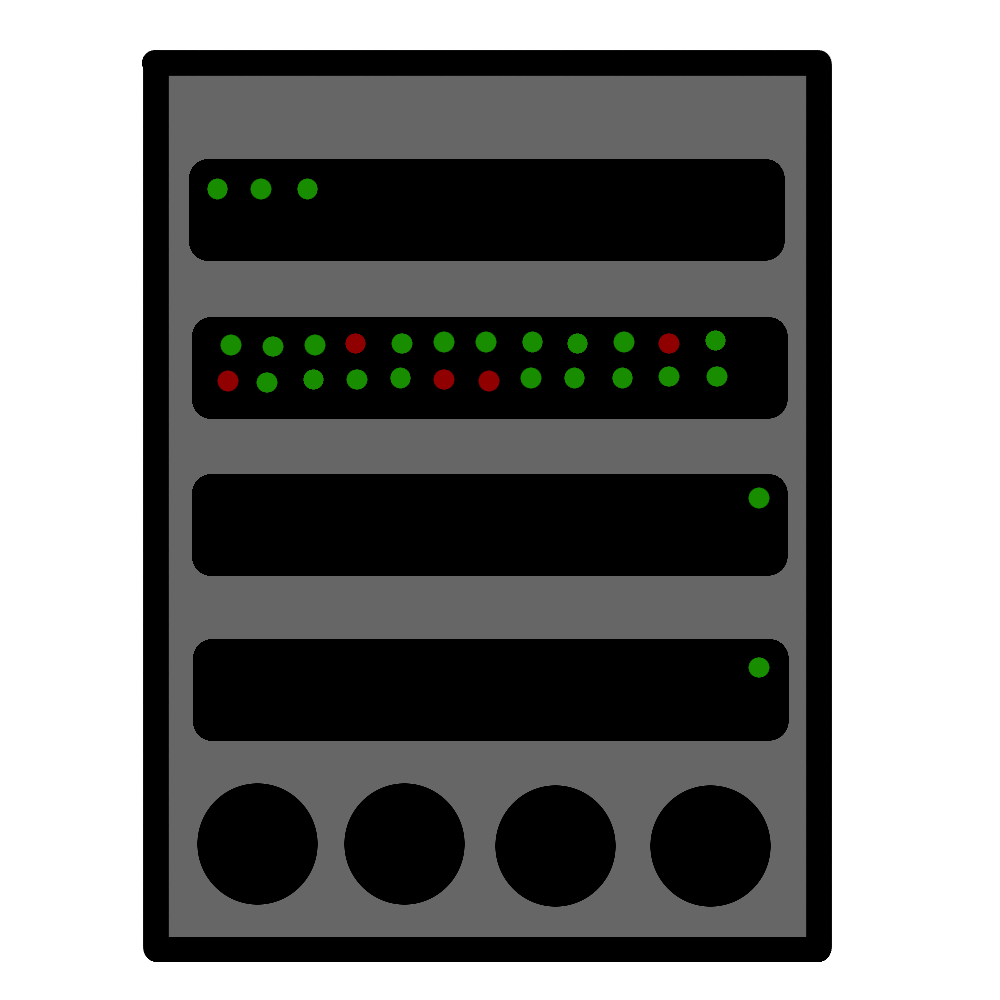
\includegraphics[width=0.5cm]{../icons/Server}}\\
            & & Sammeln, Prüfen, &\\
            & & Nonce finden, &\\
            & & \emph{\textbf{(Mining)}} &\\
        \end{tabular}
    \end{center}
\end{frame}


\begin{frame}{Fork}
    \begin{center}
        \begin{tabular}{ccccc}
            \boxwithtitle{2cm}{a}{c6cc}{...}\;\; & \boxwithtitle{2cm}{b}{aed3}{...}\;\; & \boxwithtitle{2cm}{c}{27ef}{...}\;\; & \only<2->{\boxwithtitle{2cm}{d}{fe5e}{...}\;\;} & \only<3>{\boxwithtitle{2cm}{e}{864f}{...}\;\;}\\~\\
            & & & \only<2->{\boxwithtitle{2cm}{f}{6ee6}{...}\;\;} & \\
        \end{tabular}
    \end{center}
    \begin{tikzpicture}[overlay, remember picture]
        \draw[->, line width=2pt] (b) -- (a);
        \draw[->, line width=2pt] (c) -- (b);
        \only<2->{\draw[->, line width=2pt] (d) -- (c);}
        \only<2->{\draw[->, line width=2pt] (f) -- (c);}
        \only<3->{\draw[->, line width=2pt] (e) -- (d);}
    \end{tikzpicture}
\end{frame}






% End
\section{End}
\finalslide{IT-Security}{Computational Social Choice}{Software Development \& -Architecture}

\end{document}
